\documentclass[]{IEEEtran}
% some very useful LaTeX packages include:
%\usepackage{cite}      
\usepackage{graphicx}   
\usepackage{subfigure} 
\usepackage{url}       
\usepackage{amsmath}    
\usepackage{caption2}
% Your document starts here!
\begin{document}

% Define document title and author
	\title{Weekly Report}
	\author{Adviser: Prof. Yang Wen \\Student: Cheng Wensheng\\ Period: 2018.8.27-9.2
	}
	\markboth{Visual Information Processing Group}{}
	\maketitle

% Write abstract here
\begin{abstract}
	This week I mainly put my effort on improving deep learning methods accuracy of building extraction with post processing and writing project application.
\end{abstract}

% Each section begins with a \section{title} command
\section{Sar contest}
	% \PARstart{}{} creates a tall first letter for this first paragraph
	\PARstart{S}{ince} we tried nearly all fashion neural networks of deep learning methods,	we still want to try more post processing ways to refine the output image of deep learning model.
	\begin{itemize}
		\item We tried to remove noise speckle and fill black holes in buildings last week. The result shows about 0.5$\%$ improvement, which is not obvious.
		\item This week, we use some morphology operations, like dilating and eroding to refine all building contours. This way shows some improvements on the 10 images. We handed in this version of code and waited for grading.
	\end{itemize}
	
	Fig.~\ref{fig:fw} is refined neural network result without morphology operations. Fig.~\ref{fig:rt} is the result with morphology operations.


\section{Project application}
% \PARstart{}{} creates a tall first letter for this first paragraph
\PARstart{T}{hese} two weeks, we are writing the project application of SAR image detection. This project is aimed to improve detection accuracy with simulation data and build corresponding software.
\begin{itemize}
	\item Last week, we finished the first version in short time. There are still some drawbacks, like the English characters on images, and unrelated images to SAR target.
	\item This week, we adjust structure of technical solutions and make them corresponding to key techniches. Besides, we add one research content point about simulation data and SAR image characteristic analysis.
	\item About project application, I guess it would be more efficient if Prof.Yang discusses about the whole structure with us and settle down basic items at the beginning, just like this weekend we did. In this way, we could improve our efficiency and get content to the point.
\end{itemize}


% Main Part


\newpage


\begin{figure}
	\vspace{0.5cm}
%	\begin{minipage}[t]{0.5\linewidth}
		\centering
		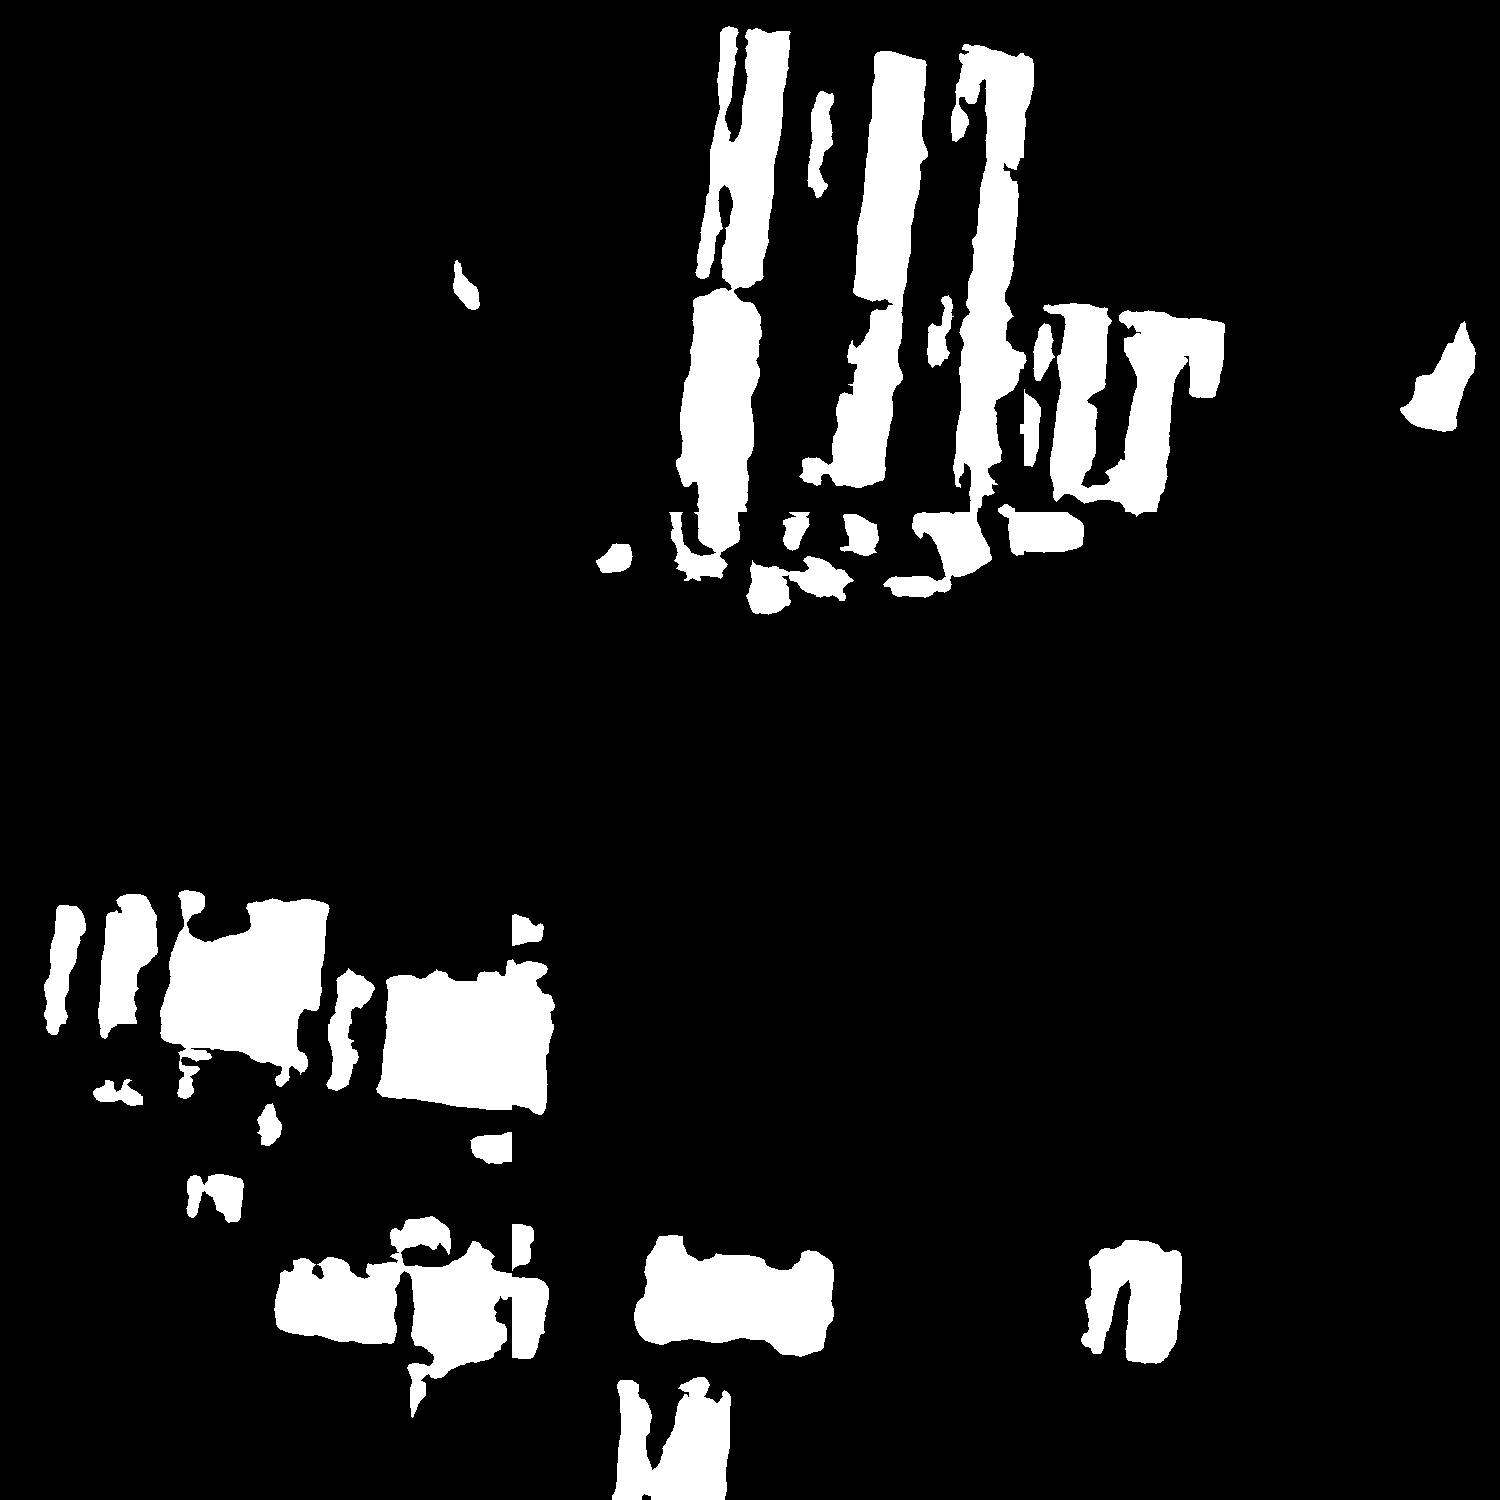
\includegraphics[width=0.7\columnwidth]{fw}
		\caption{Original result}
		\label{fig:fw}
%	\end{minipage}%
%	\begin{minipage}[t]{0.5\linewidth}
	\vspace{0.3cm}
		\centering
		
\includegraphics[width=0.7\columnwidth]{filter}
		\caption{Result with morphology operations}
		\label{fig:rt}
%	\end{minipage}
\end{figure}


%\begin{figure}[!hbt]
%%		 Center the figure.
%		\vspace{0.7cm}
%%		\hspace{50cm}
%		\begin{center}
%			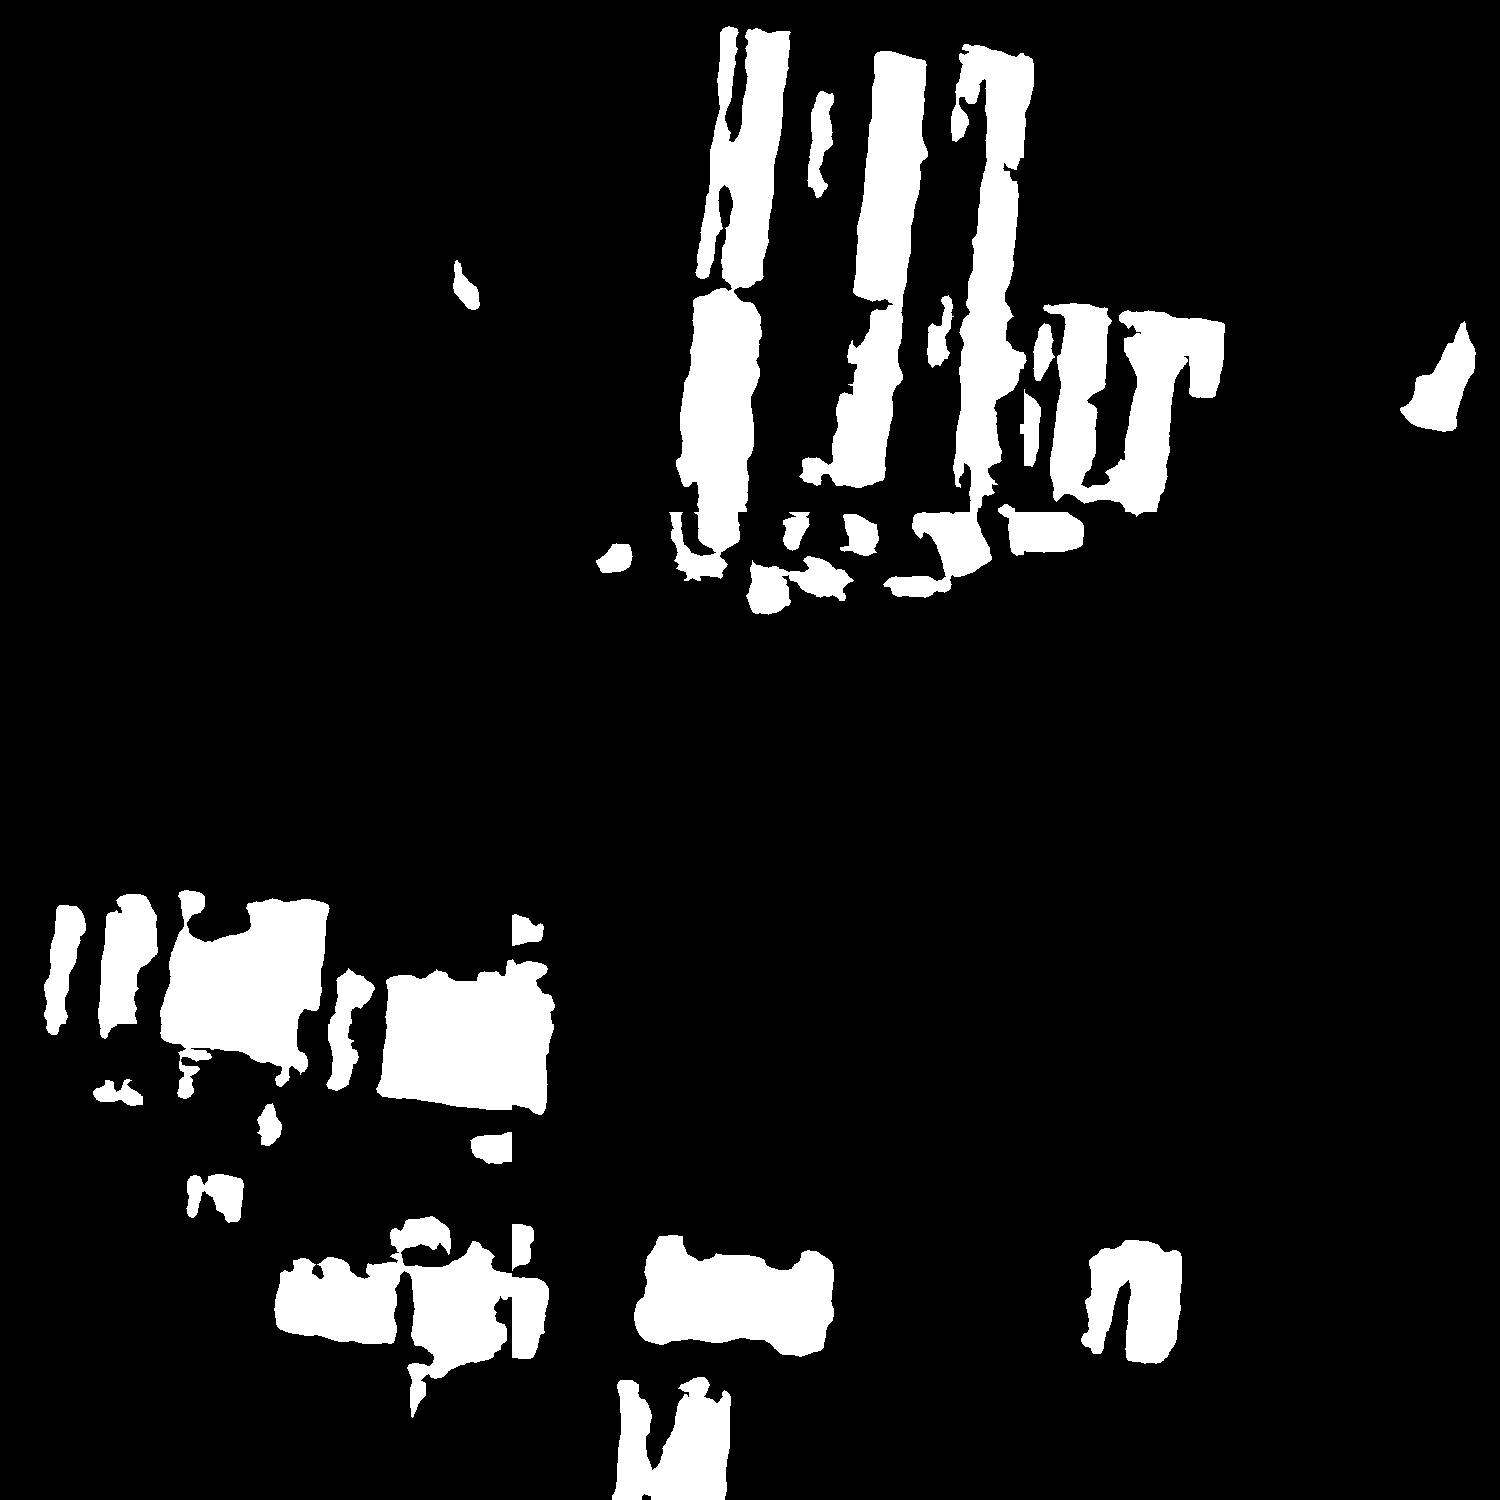
\includegraphics[width=0.2\columnwidth]{fw}
%				%		 Create a subtitle for the figure.
%			\caption{CNN methods result}
%			\label{fig:fw}
%		    \vspace{0.2cm}
%			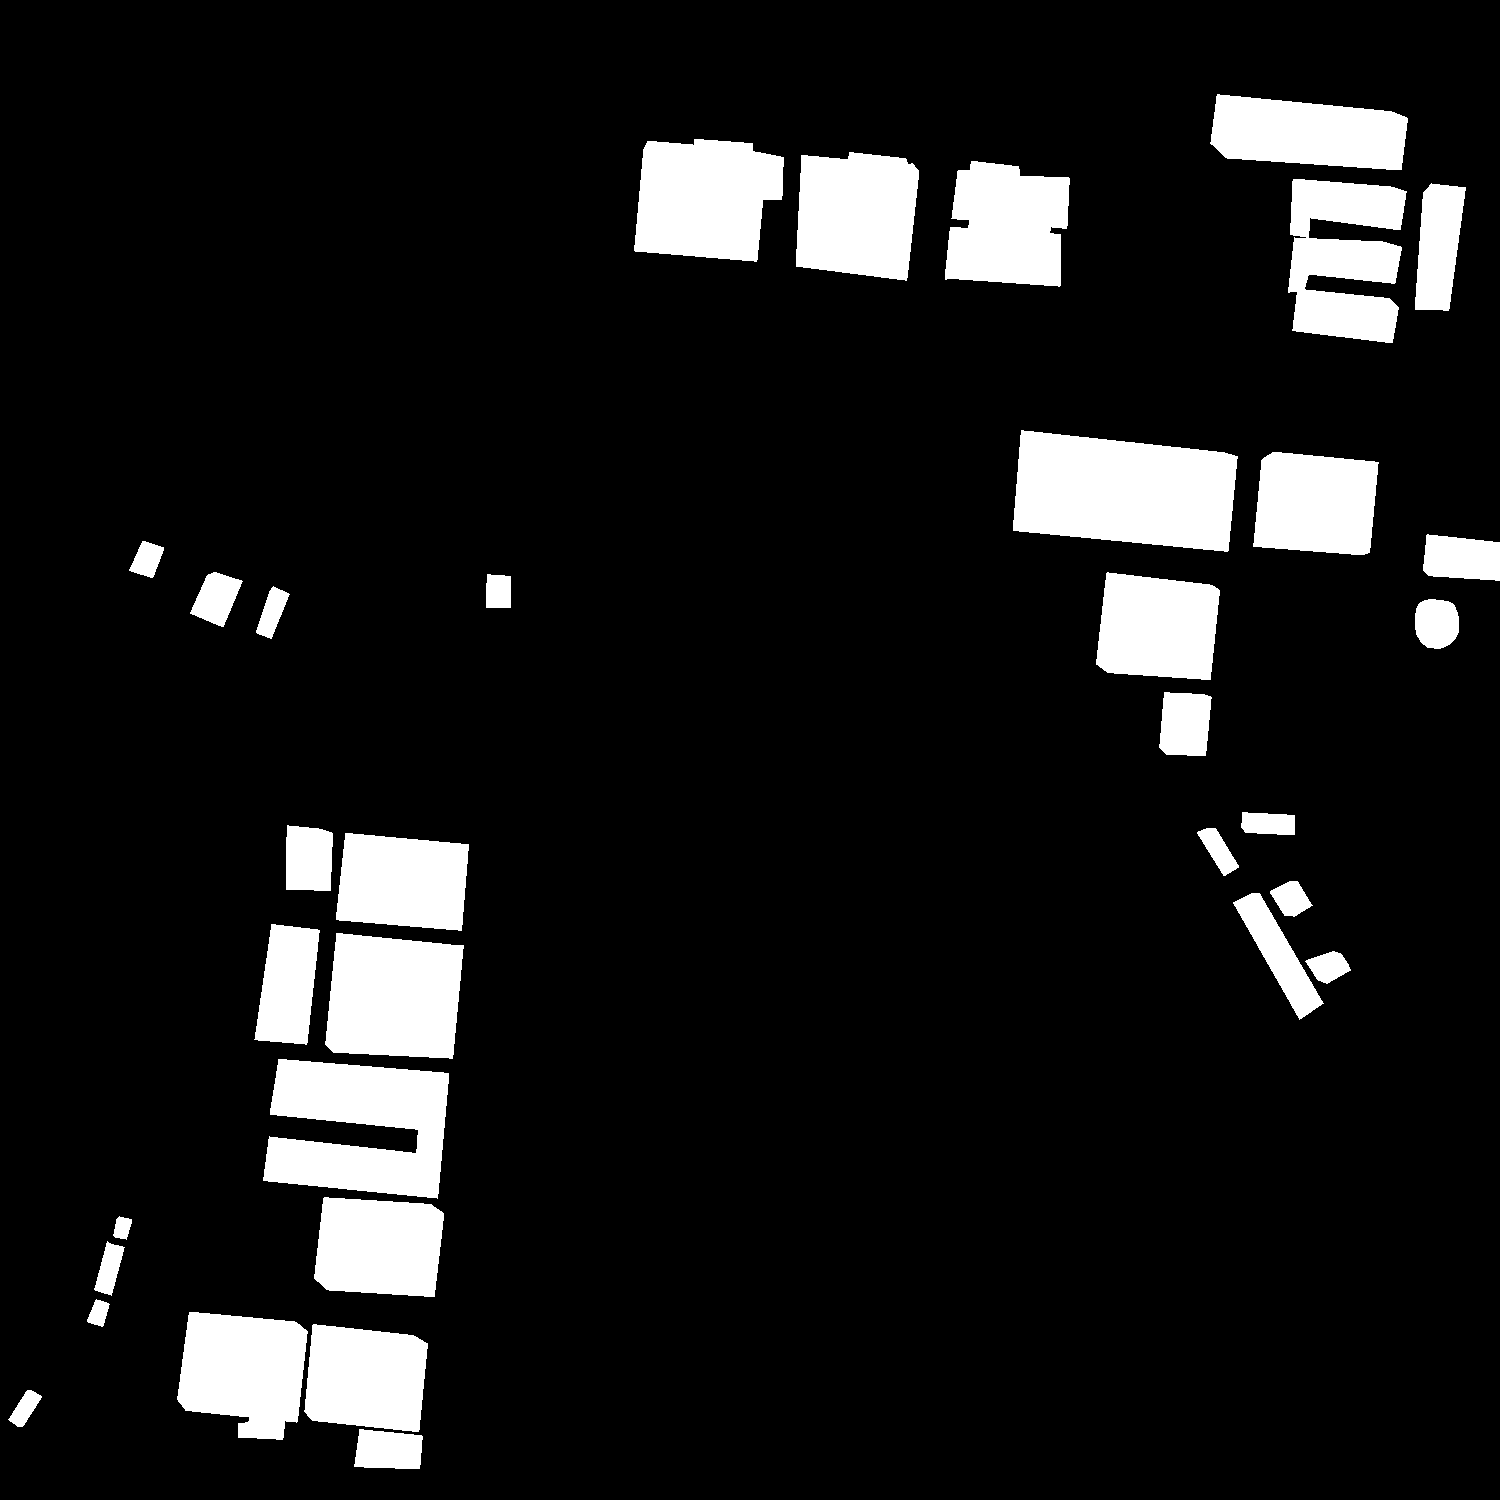
\includegraphics[width=0.2\columnwidth]{rs}
%				%Create a subtitle for the figure.
%			\caption{Ground truth}
%			\label{fig:rt}
%		\end{center}
%	\end{figure}



% Your document ends here!
\end{document}